% SPDX-FileCopyrightText: 2026 Onur Tuncer and Stereon contributors
% SPDX-License-Identifier: MPL-2.0
%
% This Source Code Form is subject to the terms of the Mozilla Public
% License, v. 2.0. If a copy of the MPL was not distributed with this
% file, You can obtain one at https://mozilla.org/MPL/2.0/.
%
% The acceptance test of display sampling (docs/meshing.rst;
% src/mesh/Sampling.cpp). A segment [t0, t1] of a polyline is kept when the
% curve's points at the seven interior eighths lie within the chord
% tolerance of the chord, and the turn between the chords of its two halves
% is within the angle tolerance; otherwise it is split at its midpoint.
\documentclass[tikz,border=6pt]{standalone}
\usepackage{amsmath}
\usetikzlibrary{calc,arrows.meta,angles,quotes}
\definecolor{curve}{RGB}{31,119,180}
\definecolor{chord}{RGB}{214,39,40}
\definecolor{half}{RGB}{44,160,44}
\begin{document}
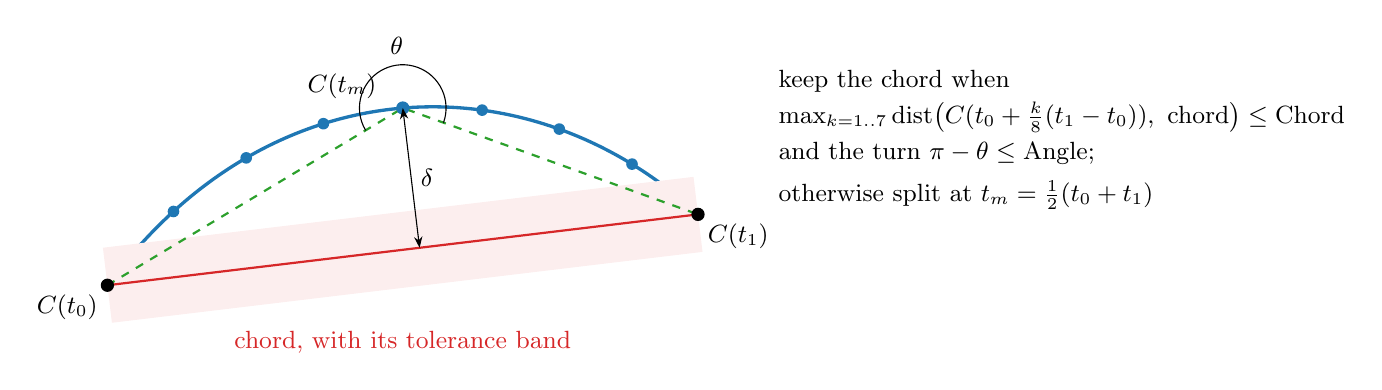
\begin{tikzpicture}[scale=1.5,lbl/.style={font=\small}]
  % The curve over the segment: a cubic through P0 and P1
  \coordinate (P0) at (0,0);
  \coordinate (P1) at (5,0.6);
  \coordinate (K1) at (1.4,1.9);
  \coordinate (K2) at (3.6,1.9);
  \draw[curve,very thick] (P0) .. controls (K1) and (K2) .. (P1);
  % The chord, and the tolerance band about it
  \fill[chord!8] ($(P0)!0.32cm!90:(P1)$) -- ($(P1)!0.32cm!-90:(P0)$)
                 -- ($(P1)!0.32cm!90:(P0)$) -- ($(P0)!0.32cm!-90:(P1)$) -- cycle;
  \draw[chord,thick] (P0) -- (P1);
  % The curve's points at t0 + k (t1 - t0) / 8, exactly on the cubic (pos is
  % its parameter); M, at k = 4, is the midpoint
  \path (P0) .. controls (K1) and (K2) .. (P1)
    \foreach \k in {1,...,7} { node[pos=\k/8] (C\k) {} };
  \coordinate (M) at (C4);
  \draw[half,thick,dashed] (P0) -- (M) -- (P1);
  % The check points
  \foreach \k in {1,2,3,5,6,7} { \fill[curve] (C\k) circle (1.4pt); }
  \fill[curve] (M) circle (1.6pt);
  % The largest distance from the chord
  \coordinate (Mfoot) at ($(P0)!(M)!(P1)$);
  \draw[{Stealth[length=4pt]}-{Stealth[length=4pt]}] (M) -- (Mfoot)
      node[lbl,midway,right] {$\delta$};
  % The turn angle at the midpoint
  \pic[draw,angle radius=0.55cm,"$\theta$",angle eccentricity=1.45,lbl] {angle=P1--M--P0};
  % Ends
  \fill (P0) circle (1.6pt) node[lbl,below left] {$C(t_0)$};
  \fill (P1) circle (1.6pt) node[lbl,below right] {$C(t_1)$};
  \node[lbl,above left,xshift=-6pt] at (M) {$C(t_m)$};
  % The test
  \node[lbl,align=left,anchor=north west] at (5.6,1.9) {%
    keep the chord when\\[2pt]
    $\max_{k=1..7} \operatorname{dist}\bigl(C(t_0 + \tfrac{k}{8}(t_1-t_0)),\ \text{chord}\bigr) \le \text{Chord}$\\[2pt]
    and the turn $\pi - \theta \le \text{Angle}$;\\[4pt]
    otherwise split at $t_m = \tfrac12(t_0 + t_1)$};
  \node[lbl,chord] at (2.5,-0.48) {chord, with its tolerance band};
\end{tikzpicture}
\end{document}
